\documentclass{standalone}
\usepackage{standalone}

\begin{document}
\subsection{FM-index}
FM-index\cite{fm_index} is the indexing implementation of Burrows-Wheeler Transform (BWT)\cite{BWT}. It is an implementation with some auxiliary data structure. Binary search is used in suffix array which would no more effective as all the columns are removed except first and last one. While compressing, it is easy to store the first column as it would be sorted. The ranks of the first columns would still be preserved as they are same as the last column. 

To match a string, suffix matching would be done here. Lets have an example, $$P = CA$$. So, the last character A should be searched in F of LF-Mapping. The next character should be occur in L and the range of that character would be found from there. Figure \ref{fig:SearchingFM} shows that for the next character C, only rank 2 and 1 is eligible to be searched. So, C should be searched in the range of of C characters in F with starting rank 2 and ending rank 1. Figure \ref{fig:SearchingFM2} shows a better illustration. As we have arrived at the begin of the string, the string exists.

The exact positions could be found using a suffix array which is a long story. Further efficiency could be gained using some auxiliary data structures. It could be shown that if a range could be found in LF-mapping, then it would be in suffix array with same length.


\begin{figure}
	\centering
	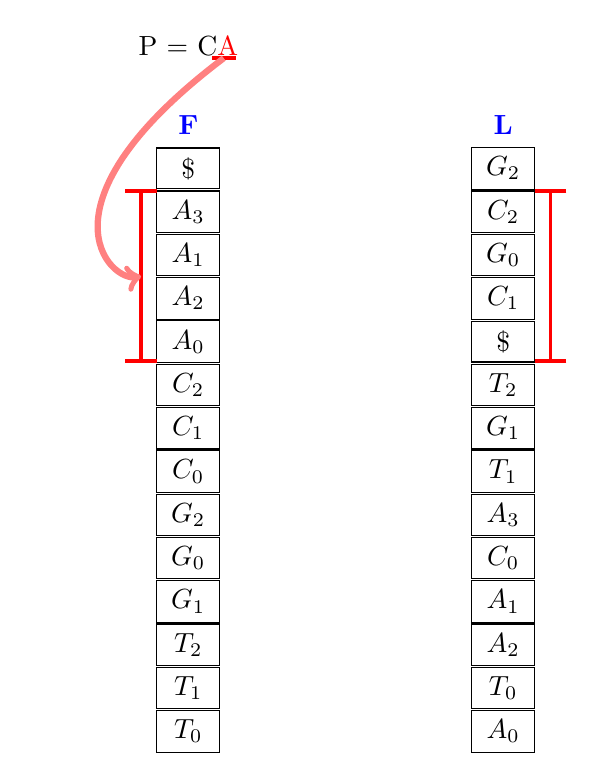
\begin{tikzpicture}[auto, node distance=5.5mm]
	% Place nodes
	\node [rectangle,color=blue,minimum width=0.8cm] (init) {\textbf{F}};
	\node [rectangle,below of=init,draw,minimum width=0.8cm] (init1) {$\$$};
	\node [rectangle,below of=init1,draw,minimum width=0.8cm] (init2) {$A_3$};
	\node [rectangle,below of=init2,draw,minimum width=0.8cm] (init3) {$A_1$};
	\node [rectangle,below of=init3,draw,minimum width=0.8cm] (init4) {$A_2$};
	\node [rectangle,below of=init4,draw,minimum width=0.8cm] (init5) {$A_0$};
	\node [rectangle,below of=init5,draw,minimum width=0.8cm] (init6) {$C_2$};
	\node [rectangle,below of=init6,draw,minimum width=0.8cm] (init7) {$C_1$};
	\node [rectangle,below of=init7,draw,minimum width=0.8cm] (init8) {$C_0$};
	\node [rectangle,below of=init8,draw,minimum width=0.8cm] (init9) {$G_2$};
	\node [rectangle,below of=init9,draw,minimum width=0.8cm] (init10) {$G_0$};
	\node [rectangle,below of=init10,draw,minimum width=0.8cm] (init111) {$G_1$};
	\node [rectangle,below of=init111,draw,minimum width=0.8cm] (init112) {$T_2$};
	\node [rectangle,below of=init112,draw,minimum width=0.8cm] (init113) {$T_1$};
	\node [rectangle,below of=init113,draw,minimum width=0.8cm] (init114) {$T_0$};
	
	\node [rectangle,color=blue,right of=init,node distance=4cm,minimum width=0.8cm] (init11) {\textbf{L}};
	\node [rectangle,below of=init11,draw,minimum width=0.8cm] (init12) {$G_2$};
	\node [rectangle,below of=init12,draw,minimum width=0.8cm] (init13) {$C_2$};
	\node [rectangle,below of=init13,draw,minimum width=0.8cm] (init14) {$G_0$};
	\node [rectangle,below of=init14,draw,minimum width=0.8cm] (init15) {$C_1$};
	\node [rectangle,below of=init15,draw,minimum width=0.8cm] (init16) {$\$$};
	\node [rectangle,below of=init16,draw,minimum width=0.8cm] (init17) {$T_2$};
	\node [rectangle,below of=init17,draw,minimum width=0.8cm] (init18) {$G_1$};
	\node [rectangle,below of=init18,draw,minimum width=0.8cm] (init19) {$T_1$};
	\node [rectangle,below of=init19,draw,minimum width=0.8cm] (init20) {$A_3$};
	\node [rectangle,below of=init20,draw,minimum width=0.8cm] (init21) {$C_0$};
	\node [rectangle,below of=init21,draw,minimum width=0.8cm] (init22) {$A_1$};
	\node [rectangle,below of=init22,draw,minimum width=0.8cm] (init23) {$A_2$};
	\node [rectangle,below of=init23,draw,minimum width=0.8cm] (init24) {$T_0$};
	\node [rectangle,below of=init24,draw,minimum width=0.8cm] (init25) {$A_0$};
	\node [rectangle] at (0,1) {P = C\textcolor{red}{A}};
	\draw [line width=0.5mm,color=red] (-0.6,-0.84) -- (-0.6,-3);
	\draw [line width=0.5mm,color=red] (-0.8,-0.84) -- (-0.4,-0.84);
	\draw [line width=0.5mm,color=red] (-0.8,-3) -- (-0.4,-3);
	
	\draw [line width=0.5mm,color=red] (4.6,-0.84) -- (4.6,-3);
	\draw [line width=0.5mm,color=red] (4.8,-0.84) -- (4.4,-0.84);
	\draw [line width=0.5mm,color=red] (4.8,-3) -- (4.4,-3);
	\draw [line width=0.5mm,color=red] (0.3,0.85) -- (0.6,0.85);
	\draw[line width=0.8mm,color=red!50,->] (0.45,0.85) .. controls(-2,-1) and (-1,-2) .. (-0.6,-1.92);
	\end{tikzpicture}
	\caption{Finding Suffix A of Query String P in F of LF Mapping.}
	\label{fig:SearchingFM}
\end{figure}
\begin{figure}
	\centering
	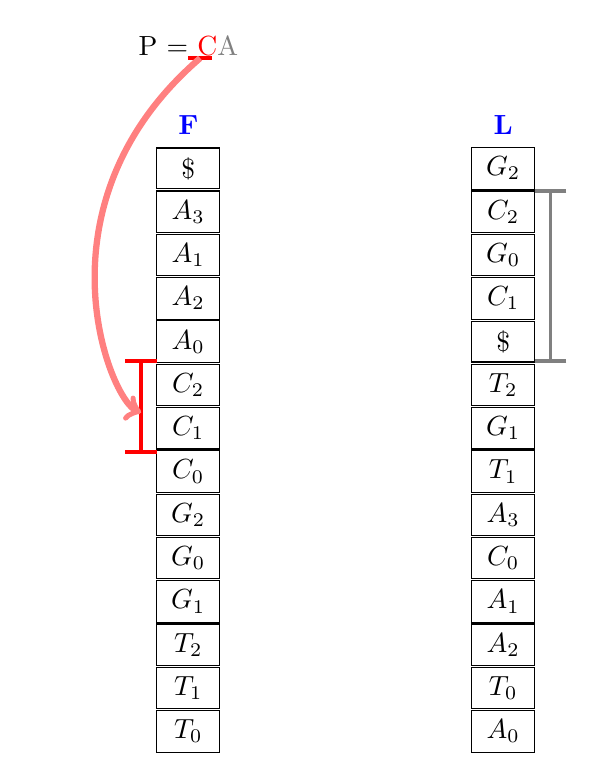
\begin{tikzpicture}[auto, node distance=5.5mm]
	% Place nodes
	\node [rectangle,color=blue,minimum width=0.8cm] (init) {\textbf{F}};
	\node [rectangle,below of=init,draw,minimum width=0.8cm] (init1) {$\$$};
	\node [rectangle,below of=init1,draw,minimum width=0.8cm] (init2) {$A_3$};
	\node [rectangle,below of=init2,draw,minimum width=0.8cm] (init3) {$A_1$};
	\node [rectangle,below of=init3,draw,minimum width=0.8cm] (init4) {$A_2$};
	\node [rectangle,below of=init4,draw,minimum width=0.8cm] (init5) {$A_0$};
	\node [rectangle,below of=init5,draw,minimum width=0.8cm] (init6) {$C_2$};
	\node [rectangle,below of=init6,draw,minimum width=0.8cm] (init7) {$C_1$};
	\node [rectangle,below of=init7,draw,minimum width=0.8cm] (init8) {$C_0$};
	\node [rectangle,below of=init8,draw,minimum width=0.8cm] (init9) {$G_2$};
	\node [rectangle,below of=init9,draw,minimum width=0.8cm] (init10) {$G_0$};
	\node [rectangle,below of=init10,draw,minimum width=0.8cm] (init111) {$G_1$};
	\node [rectangle,below of=init111,draw,minimum width=0.8cm] (init112) {$T_2$};
	\node [rectangle,below of=init112,draw,minimum width=0.8cm] (init113) {$T_1$};
	\node [rectangle,below of=init113,draw,minimum width=0.8cm] (init114) {$T_0$};
	
	\node [rectangle,color=blue,right of=init,node distance=4cm,minimum width=0.8cm] (init11) {\textbf{L}};
	\node [rectangle,below of=init11,draw,minimum width=0.8cm] (init12) {$G_2$};
	\node [rectangle,below of=init12,draw,minimum width=0.8cm] (init13) {$C_2$};
	\node [rectangle,below of=init13,draw,minimum width=0.8cm] (init14) {$G_0$};
	\node [rectangle,below of=init14,draw,minimum width=0.8cm] (init15) {$C_1$};
	\node [rectangle,below of=init15,draw,minimum width=0.8cm] (init16) {$\$$};
	\node [rectangle,below of=init16,draw,minimum width=0.8cm] (init17) {$T_2$};
	\node [rectangle,below of=init17,draw,minimum width=0.8cm] (init18) {$G_1$};
	\node [rectangle,below of=init18,draw,minimum width=0.8cm] (init19) {$T_1$};
	\node [rectangle,below of=init19,draw,minimum width=0.8cm] (init20) {$A_3$};
	\node [rectangle,below of=init20,draw,minimum width=0.8cm] (init21) {$C_0$};
	\node [rectangle,below of=init21,draw,minimum width=0.8cm] (init22) {$A_1$};
	\node [rectangle,below of=init22,draw,minimum width=0.8cm] (init23) {$A_2$};
	\node [rectangle,below of=init23,draw,minimum width=0.8cm] (init24) {$T_0$};
	\node [rectangle,below of=init24,draw,minimum width=0.8cm] (init25) {$A_0$};
	\node [rectangle] at (0,1) {P = \textcolor{red}{C}\textcolor{black!50}{A}};
	\draw [line width=0.5mm,color=red] (-0.6,-4.15) -- (-0.6,-3);
	\draw [line width=0.5mm,color=red] (-0.8,-4.15) -- (-0.4,-4.15);
	\draw [line width=0.5mm,color=red] (-0.8,-3) -- (-0.4,-3);
	
	\draw [line width=0.5mm,color=black!50] (4.6,-0.84) -- (4.6,-3);
	\draw [line width=0.5mm,color=black!50] (4.8,-0.84) -- (4.4,-0.84);
	\draw [line width=0.5mm,color=black!50] (4.8,-3) -- (4.4,-3);
	
	\draw [line width=0.5mm,color=red] (0,0.85) -- (0.3,0.85);
	
	\draw[line width=0.8mm,color=red!50,->] (0.15,0.85) .. controls(-2,-1) and (-1,-3.5) .. (-0.6,-3.65);
	\end{tikzpicture}
	\caption{Finding Suffix C of Query String P in F of LF Mapping.}
	\label{fig:SearchingFM2}
\end{figure}
\end{document}